\documentclass[1p]{elsarticle_modified}
%\bibliographystyle{elsarticle-num}

%\usepackage[colorlinks]{hyperref}
%\usepackage{abbrmath_seonhwa} %\Abb, \Ascr, \Acal ,\Abf, \Afrak
\usepackage{amsfonts}
\usepackage{amssymb}
\usepackage{amsmath}
\usepackage{amsthm}
\usepackage{scalefnt}
\usepackage{amsbsy}
\usepackage{kotex}
\usepackage{caption}
\usepackage{subfig}
\usepackage{color}
\usepackage{graphicx}
\usepackage{xcolor} %% white, black, red, green, blue, cyan, magenta, yellow
\usepackage{float}
\usepackage{setspace}
\usepackage{hyperref}

\usepackage{tikz}
\usetikzlibrary{arrows}

\usepackage{multirow}
\usepackage{array} % fixed length table
\usepackage{hhline}

%%%%%%%%%%%%%%%%%%%%%
\makeatletter
\renewcommand*\env@matrix[1][\arraystretch]{%
	\edef\arraystretch{#1}%
	\hskip -\arraycolsep
	\let\@ifnextchar\new@ifnextchar
	\array{*\c@MaxMatrixCols c}}
\makeatother %https://tex.stackexchange.com/questions/14071/how-can-i-increase-the-line-spacing-in-a-matrix
%%%%%%%%%%%%%%%

\usepackage[normalem]{ulem}

\newcommand{\msout}[1]{\ifmmode\text{\sout{\ensuremath{#1}}}\else\sout{#1}\fi}
%SOURCE: \msout is \stkout macro in https://tex.stackexchange.com/questions/20609/strikeout-in-math-mode

\newcommand{\cancel}[1]{
	\ifmmode
	{\color{red}\msout{#1}}
	\else
	{\color{red}\sout{#1}}
	\fi
}

\newcommand{\add}[1]{
	{\color{blue}\uwave{#1}}
}

\newcommand{\replace}[2]{
	\ifmmode
	{\color{red}\msout{#1}}{\color{blue}\uwave{#2}}
	\else
	{\color{red}\sout{#1}}{\color{blue}\uwave{#2}}
	\fi
}

\newcommand{\Sol}{\mathcal{S}} %segment
\newcommand{\D}{D} %diagram
\newcommand{\A}{\mathcal{A}} %arc


%%%%%%%%%%%%%%%%%%%%%%%%%%%%%5 test

\def\sl{\operatorname{\textup{SL}}(2,\Cbb)}
\def\psl{\operatorname{\textup{PSL}}(2,\Cbb)}
\def\quan{\mkern 1mu \triangleright \mkern 1mu}

\theoremstyle{definition}
\newtheorem{thm}{Theorem}[section]
\newtheorem{prop}[thm]{Proposition}
\newtheorem{lem}[thm]{Lemma}
\newtheorem{ques}[thm]{Question}
\newtheorem{cor}[thm]{Corollary}
\newtheorem{defn}[thm]{Definition}
\newtheorem{exam}[thm]{Example}
\newtheorem{rmk}[thm]{Remark}
\newtheorem{alg}[thm]{Algorithm}

\newcommand{\I}{\sqrt{-1}}
\begin{document}

%\begin{frontmatter}
%
%\title{Boundary parabolic representations of knots up to 8 crossings}
%
%%% Group authors per affiliation:
%\author{Yunhi Cho} 
%\address{Department of Mathematics, University of Seoul, Seoul, Korea}
%\ead{yhcho@uos.ac.kr}
%
%
%\author{Seonhwa Kim} %\fnref{s_kim}}
%\address{Center for Geometry and Physics, Institute for Basic Science, Pohang, 37673, Korea}
%\ead{ryeona17@ibs.re.kr}
%
%\author{Hyuk Kim}
%\address{Department of Mathematical Sciences, Seoul National University, Seoul 08826, Korea}
%\ead{hyukkim@snu.ac.kr}
%
%\author{Seokbeom Yoon}
%\address{Department of Mathematical Sciences, Seoul National University, Seoul, 08826,  Korea}
%\ead{sbyoon15@snu.ac.kr}
%
%\begin{abstract}
%We find all boundary parabolic representation of knots up to 8 crossings.
%
%\end{abstract}
%\begin{keyword}
%    \MSC[2010] 57M25 
%\end{keyword}
%
%\end{frontmatter}

%\linenumbers
%\tableofcontents
%
\newcommand\colored[1]{\textcolor{white}{\rule[-0.35ex]{0.8em}{1.4ex}}\kern-0.8em\color{red} #1}%
%\newcommand\colored[1]{\textcolor{white}{ #1}\kern-2.17ex	\textcolor{white}{ #1}\kern-1.81ex	\textcolor{white}{ #1}\kern-2.15ex\color{red}#1	}

{\Large $\underline{12n_{0594}~(K12n_{0594})}$}

\setlength{\tabcolsep}{10pt}
\renewcommand{\arraystretch}{1.6}
\vspace{1cm}\begin{tabular}{m{100pt}>{\centering\arraybackslash}m{274pt}}
\multirow{5}{120pt}{
	\centering
	\includegraphics[width=112pt]{../../../GIT/diagram.site/Diagrams/png/2683_12n_0594.png}\\
\ \ \ A knot diagram\footnotemark}&
\allowdisplaybreaks
\textbf{Linearized knot diagam} \\
\cline{2-2}
 &
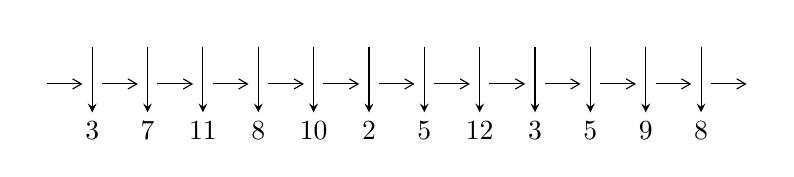
\begin{tikzpicture}[x=20pt, y=17pt]
	% nodes
	\node (C0) at (0, 0) {};
	\node (C1) at (1, 0) {};
	\node (C1U) at (1, +1) {};
	\node (C1D) at (1, -1) {3};

	\node (C2) at (2, 0) {};
	\node (C2U) at (2, +1) {};
	\node (C2D) at (2, -1) {7};

	\node (C3) at (3, 0) {};
	\node (C3U) at (3, +1) {};
	\node (C3D) at (3, -1) {11};

	\node (C4) at (4, 0) {};
	\node (C4U) at (4, +1) {};
	\node (C4D) at (4, -1) {8};

	\node (C5) at (5, 0) {};
	\node (C5U) at (5, +1) {};
	\node (C5D) at (5, -1) {10};

	\node (C6) at (6, 0) {};
	\node (C6U) at (6, +1) {};
	\node (C6D) at (6, -1) {2};

	\node (C7) at (7, 0) {};
	\node (C7U) at (7, +1) {};
	\node (C7D) at (7, -1) {5};

	\node (C8) at (8, 0) {};
	\node (C8U) at (8, +1) {};
	\node (C8D) at (8, -1) {12};

	\node (C9) at (9, 0) {};
	\node (C9U) at (9, +1) {};
	\node (C9D) at (9, -1) {3};

	\node (C10) at (10, 0) {};
	\node (C10U) at (10, +1) {};
	\node (C10D) at (10, -1) {5};

	\node (C11) at (11, 0) {};
	\node (C11U) at (11, +1) {};
	\node (C11D) at (11, -1) {9};

	\node (C12) at (12, 0) {};
	\node (C12U) at (12, +1) {};
	\node (C12D) at (12, -1) {8};
	\node (C13) at (13, 0) {};

	% arrows
	\draw[->,>={angle 60}]
	(C0) edge (C1) (C1) edge (C2) (C2) edge (C3) (C3) edge (C4) (C4) edge (C5) (C5) edge (C6) (C6) edge (C7) (C7) edge (C8) (C8) edge (C9) (C9) edge (C10) (C10) edge (C11) (C11) edge (C12) (C12) edge (C13) ;	\draw[->,>=stealth]
	(C1U) edge (C1D) (C2U) edge (C2D) (C3U) edge (C3D) (C4U) edge (C4D) (C5U) edge (C5D) (C6U) edge (C6D) (C7U) edge (C7D) (C8U) edge (C8D) (C9U) edge (C9D) (C10U) edge (C10D) (C11U) edge (C11D) (C12U) edge (C12D) ;
	\end{tikzpicture} \\
\hhline{~~} \\& 
\textbf{Solving Sequence} \\ \cline{2-2} 
 &
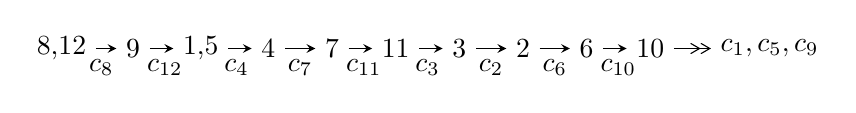
\begin{tikzpicture}[x=23pt, y=7pt]
	% node
	\node (A0) at (-1/8, 0) {8,12};
	\node (A1) at (1, 0) {9};
	\node (A2) at (33/16, 0) {1,5};
	\node (A3) at (25/8, 0) {4};
	\node (A4) at (33/8, 0) {7};
	\node (A5) at (41/8, 0) {11};
	\node (A6) at (49/8, 0) {3};
	\node (A7) at (57/8, 0) {2};
	\node (A8) at (65/8, 0) {6};
	\node (A9) at (73/8, 0) {10};
	\node (C1) at (1/2, -1) {$c_{8}$};
	\node (C2) at (3/2, -1) {$c_{12}$};
	\node (C3) at (21/8, -1) {$c_{4}$};
	\node (C4) at (29/8, -1) {$c_{7}$};
	\node (C5) at (37/8, -1) {$c_{11}$};
	\node (C6) at (45/8, -1) {$c_{3}$};
	\node (C7) at (53/8, -1) {$c_{2}$};
	\node (C8) at (61/8, -1) {$c_{6}$};
	\node (C9) at (69/8, -1) {$c_{10}$};
	\node (A10) at (11, 0) {$c_{1},c_{5},c_{9}$};

	% edge
	\draw[->,>=stealth]	
	(A0) edge (A1) (A1) edge (A2) (A2) edge (A3) (A3) edge (A4) (A4) edge (A5) (A5) edge (A6) (A6) edge (A7) (A7) edge (A8) (A8) edge (A9) ;
	\draw[->>,>={angle 60}]	
	(A9) edge (A10);
\end{tikzpicture} \\ 

\end{tabular} \\

\footnotetext{
The image of knot diagram is generated by the software ``\textbf{Draw programme}" developed by Andrew Bartholomew(\url{http://www.layer8.co.uk/maths/draw/index.htm\#Running-draw}), where we modified some parts for our purpose(\url{https://github.com/CATsTAILs/LinksPainter}).
}\phantom \\ \newline 
\centering \textbf{Ideals for irreducible components\footnotemark of $X_{\text{par}}$} 
 
\begin{align*}
I^u_{1}&=\langle 
-4 u^{19}-11 u^{18}+\cdots+b-6,\;-2 u^{19}-3 u^{18}+\cdots+a-7,\;u^{20}+3 u^{19}+\cdots+3 u+1\rangle \\
I^u_{2}&=\langle 
-2 u^{13}+8 u^{12}+\cdots+b+3,\\
\phantom{I^u_{2}}&\phantom{= \langle  }- u^{13}+2 u^{12}-6 u^{11}+7 u^{10}-10 u^9+8 u^8-4 u^7+4 u^6+3 u^5+2 u^4+2 u^3-2 u^2+a-2,\\
\phantom{I^u_{2}}&\phantom{= \langle  }u^{14}-4 u^{13}+13 u^{12}-28 u^{11}+50 u^{10}-72 u^9+86 u^8-89 u^7+76 u^6-59 u^5+39 u^4-23 u^3+12 u^2-4 u+1\rangle \\
\\
\end{align*}
\raggedright * 2 irreducible components of $\dim_{\mathbb{C}}=0$, with total 34 representations.\\
\footnotetext{All coefficients of polynomials are rational numbers. But the coefficients are sometimes approximated in decimal forms when there is not enough margin.}
\newpage
\renewcommand{\arraystretch}{1}
\centering \section*{I. $I^u_{1}= \langle -4 u^{19}-11 u^{18}+\cdots+b-6,\;-2 u^{19}-3 u^{18}+\cdots+a-7,\;u^{20}+3 u^{19}+\cdots+3 u+1 \rangle$}
\flushleft \textbf{(i) Arc colorings}\\
\begin{tabular}{m{7pt} m{180pt} m{7pt} m{180pt} }
\flushright $a_{8}=$&$\begin{pmatrix}1\\0\end{pmatrix}$ \\
\flushright $a_{12}=$&$\begin{pmatrix}0\\u\end{pmatrix}$ \\
\flushright $a_{9}=$&$\begin{pmatrix}1\\u^2\end{pmatrix}$ \\
\flushright $a_{1}=$&$\begin{pmatrix}- u\\u\end{pmatrix}$ \\
\flushright $a_{5}=$&$\begin{pmatrix}2 u^{19}+3 u^{18}+\cdots- u+7\\4 u^{19}+11 u^{18}+\cdots+5 u+6\end{pmatrix}$ \\
\flushright $a_{4}=$&$\begin{pmatrix}6 u^{19}+14 u^{18}+\cdots+4 u+13\\4 u^{19}+11 u^{18}+\cdots+5 u+6\end{pmatrix}$ \\
\flushright $a_{7}=$&$\begin{pmatrix}- u^{19}- u^{18}+\cdots- u+1\\- u^{19}-4 u^{18}+\cdots-4 u-2\end{pmatrix}$ \\
\flushright $a_{11}=$&$\begin{pmatrix}u\\u^3+u\end{pmatrix}$ \\
\flushright $a_{3}=$&$\begin{pmatrix}3 u^{19}+7 u^{18}+\cdots+4 u+12\\4 u^{19}+10 u^{18}+\cdots+2 u+3\end{pmatrix}$ \\
\flushright $a_{2}=$&$\begin{pmatrix}u^{19}+u^{18}+\cdots+2 u+1\\u^{19}+4 u^{18}+\cdots+4 u+1\end{pmatrix}$ \\
\flushright $a_{6}=$&$\begin{pmatrix}-2 u^{19}-2 u^{18}+\cdots+3 u-6\\-4 u^{19}-12 u^{18}+\cdots-5 u-6\end{pmatrix}$ \\
\flushright $a_{10}=$&$\begin{pmatrix}u^{18}+2 u^{17}+\cdots+2 u+1\\- u^{19}-3 u^{18}+\cdots-2 u-1\end{pmatrix}$\\&\end{tabular}
\flushleft \textbf{(ii) Obstruction class $= -1$}\\~\\
\flushleft \textbf{(iii) Cusp Shapes $= 20 u^{19}+55 u^{18}+219 u^{17}+423 u^{16}+917 u^{15}+1354 u^{14}+1901 u^{13}+2075 u^{12}+1606 u^{11}+752 u^{10}-1039 u^9-2337 u^8-3525 u^7-3656 u^6-2870 u^5-1973 u^4-773 u^3-277 u^2+20 u+23$}\\~\\
\newpage\renewcommand{\arraystretch}{1}
\flushleft \textbf{(iv) u-Polynomials at the component}\newline \\
\begin{tabular}{m{50pt}|m{274pt}}
Crossings & \hspace{64pt}u-Polynomials at each crossing \\
\hline $$\begin{aligned}c_{1}\end{aligned}$$&$\begin{aligned}
&u^{20}+10 u^{19}+\cdots+29696 u+4096
\end{aligned}$\\
\hline $$\begin{aligned}c_{2},c_{6}\end{aligned}$$&$\begin{aligned}
&u^{20}-16 u^{19}+\cdots+224 u-64
\end{aligned}$\\
\hline $$\begin{aligned}c_{3}\end{aligned}$$&$\begin{aligned}
&u^{20}+2 u^{19}+\cdots-135 u-31
\end{aligned}$\\
\hline $$\begin{aligned}c_{4},c_{7}\end{aligned}$$&$\begin{aligned}
&u^{20}-4 u^{19}+\cdots+u-1
\end{aligned}$\\
\hline $$\begin{aligned}c_{5},c_{9},c_{10}\end{aligned}$$&$\begin{aligned}
&u^{20}- u^{19}+\cdots-3 u-1
\end{aligned}$\\
\hline $$\begin{aligned}c_{8},c_{11},c_{12}\end{aligned}$$&$\begin{aligned}
&u^{20}-3 u^{19}+\cdots-3 u+1
\end{aligned}$\\
\hline
\end{tabular}\\~\\
\newpage\renewcommand{\arraystretch}{1}
\flushleft \textbf{(v) Riley Polynomials at the component}\newline \\
\begin{tabular}{m{50pt}|m{274pt}}
Crossings & \hspace{64pt}Riley Polynomials at each crossing \\
\hline $$\begin{aligned}c_{1}\end{aligned}$$&$\begin{aligned}
&y^{20}+102 y^{19}+\cdots-1112539136 y+16777216
\end{aligned}$\\
\hline $$\begin{aligned}c_{2},c_{6}\end{aligned}$$&$\begin{aligned}
&y^{20}-10 y^{19}+\cdots-29696 y+4096
\end{aligned}$\\
\hline $$\begin{aligned}c_{3}\end{aligned}$$&$\begin{aligned}
&y^{20}+44 y^{19}+\cdots-12831 y+961
\end{aligned}$\\
\hline $$\begin{aligned}c_{4},c_{7}\end{aligned}$$&$\begin{aligned}
&y^{20}+42 y^{19}+\cdots-29 y+1
\end{aligned}$\\
\hline $$\begin{aligned}c_{5},c_{9},c_{10}\end{aligned}$$&$\begin{aligned}
&y^{20}+49 y^{19}+\cdots+9 y+1
\end{aligned}$\\
\hline $$\begin{aligned}c_{8},c_{11},c_{12}\end{aligned}$$&$\begin{aligned}
&y^{20}+15 y^{19}+\cdots-21 y+1
\end{aligned}$\\
\hline
\end{tabular}\\~\\
\newpage\flushleft \textbf{(vi) Complex Volumes and Cusp Shapes}
$$\begin{array}{c|c|c}  
\text{Solutions to }I^u_{1}& \I (\text{vol} + \sqrt{-1}CS) & \text{Cusp shape}\\
 \hline 
\begin{aligned}
u &= -1.042660 + 0.036790 I \\
a &= -0.041706 - 0.146779 I \\
b &= -1.09913 + 2.60338 I\end{aligned}
 & \phantom{-}15.4500 + 5.4797 I & -10.60978 - 2.00835 I \\ \hline\begin{aligned}
u &= -1.042660 - 0.036790 I \\
a &= -0.041706 + 0.146779 I \\
b &= -1.09913 - 2.60338 I\end{aligned}
 & \phantom{-}15.4500 - 5.4797 I & -10.60978 + 2.00835 I \\ \hline\begin{aligned}
u &= \phantom{-}1.08731\phantom{ +0.000000I} \\
a &= \phantom{-}0.282292\phantom{ +0.000000I} \\
b &= -0.147050\phantom{ +0.000000I}\end{aligned}
 & -5.86045\phantom{ +0.000000I} & -4.92500\phantom{ +0.000000I} \\ \hline\begin{aligned}
u &= -0.176041 + 0.850242 I \\
a &= -0.272973 + 1.045810 I \\
b &= \phantom{-}0.746840 - 0.265541 I\end{aligned}
 & -0.414648 + 1.016570 I & -12.17893 - 0.72142 I \\ \hline\begin{aligned}
u &= -0.176041 - 0.850242 I \\
a &= -0.272973 - 1.045810 I \\
b &= \phantom{-}0.746840 + 0.265541 I\end{aligned}
 & -0.414648 - 1.016570 I & -12.17893 + 0.72142 I \\ \hline\begin{aligned}
u &= \phantom{-}0.222003 + 1.123880 I \\
a &= -0.155980 - 0.668566 I \\
b &= -0.185769 + 0.435768 I\end{aligned}
 & \phantom{-}2.27216 - 2.01728 I & -6.94050 + 3.50947 I \\ \hline\begin{aligned}
u &= \phantom{-}0.222003 - 1.123880 I \\
a &= -0.155980 + 0.668566 I \\
b &= -0.185769 - 0.435768 I\end{aligned}
 & \phantom{-}2.27216 + 2.01728 I & -6.94050 - 3.50947 I \\ \hline\begin{aligned}
u &= -0.153005 + 1.219290 I \\
a &= \phantom{-}0.53928 + 1.84965 I \\
b &= \phantom{-}0.69118 - 1.43719 I\end{aligned}
 & \phantom{-}5.80153 + 4.79888 I & -3.91055 - 4.91239 I \\ \hline\begin{aligned}
u &= -0.153005 - 1.219290 I \\
a &= \phantom{-}0.53928 - 1.84965 I \\
b &= \phantom{-}0.69118 + 1.43719 I\end{aligned}
 & \phantom{-}5.80153 - 4.79888 I & -3.91055 + 4.91239 I \\ \hline\begin{aligned}
u &= -0.112420 + 1.234960 I \\
a &= -0.73519 - 1.51536 I \\
b &= -0.356045 + 1.326390 I\end{aligned}
 & \phantom{-}6.14605 - 0.99742 I & -6.22294 + 0.30113 I\\
 \hline 
 \end{array}$$\newpage$$\begin{array}{c|c|c}  
\text{Solutions to }I^u_{1}& \I (\text{vol} + \sqrt{-1}CS) & \text{Cusp shape}\\
 \hline 
\begin{aligned}
u &= -0.112420 - 1.234960 I \\
a &= -0.73519 + 1.51536 I \\
b &= -0.356045 - 1.326390 I\end{aligned}
 & \phantom{-}6.14605 + 0.99742 I & -6.22294 - 0.30113 I \\ \hline\begin{aligned}
u &= \phantom{-}0.538721 + 1.305800 I \\
a &= \phantom{-}0.121911 + 0.351718 I \\
b &= \phantom{-}0.036915 - 0.257923 I\end{aligned}
 & -1.83437 - 5.75000 I & -9.64448 - 0.35618 I \\ \hline\begin{aligned}
u &= \phantom{-}0.538721 - 1.305800 I \\
a &= \phantom{-}0.121911 - 0.351718 I \\
b &= \phantom{-}0.036915 + 0.257923 I\end{aligned}
 & -1.83437 + 5.75000 I & -9.64448 + 0.35618 I \\ \hline\begin{aligned}
u &= -0.54565 + 1.32924 I \\
a &= \phantom{-}2.33430 + 1.17622 I \\
b &= -1.00453 - 2.47780 I\end{aligned}
 & \phantom{-}19.4483 + 0.1620 I & -7.85194 - 0.70320 I \\ \hline\begin{aligned}
u &= -0.54565 - 1.32924 I \\
a &= \phantom{-}2.33430 - 1.17622 I \\
b &= -1.00453 + 2.47780 I\end{aligned}
 & \phantom{-}19.4483 - 0.1620 I & -7.85194 + 0.70320 I \\ \hline\begin{aligned}
u &= -0.50245 + 1.36268 I \\
a &= -0.91739 - 2.80304 I \\
b &= -1.11454 + 2.73435 I\end{aligned}
 & -19.6493 + 10.9702 I & -7.71994 - 4.45500 I \\ \hline\begin{aligned}
u &= -0.50245 - 1.36268 I \\
a &= -0.91739 + 2.80304 I \\
b &= -1.11454 - 2.73435 I\end{aligned}
 & -19.6493 - 10.9702 I & -7.71994 + 4.45500 I \\ \hline\begin{aligned}
u &= -0.401727 + 0.043777 I \\
a &= \phantom{-}0.05735 + 1.66973 I \\
b &= \phantom{-}0.241130 + 1.099340 I\end{aligned}
 & \phantom{-}2.31319 - 2.74078 I & -11.17617 + 6.82485 I \\ \hline\begin{aligned}
u &= -0.401727 - 0.043777 I \\
a &= \phantom{-}0.05735 - 1.66973 I \\
b &= \phantom{-}0.241130 - 1.099340 I\end{aligned}
 & \phantom{-}2.31319 + 2.74078 I & -11.17617 - 6.82485 I \\ \hline\begin{aligned}
u &= \phantom{-}0.259155\phantom{ +0.000000I} \\
a &= -1.14150\phantom{ +0.000000I} \\
b &= \phantom{-}0.234939\phantom{ +0.000000I}\end{aligned}
 & -0.567617\phantom{ +0.000000I} & -17.5650\phantom{ +0.000000I}\\
 \hline 
 \end{array}$$\newpage\newpage\renewcommand{\arraystretch}{1}
\centering \section*{II. $I^u_{2}= \langle -2 u^{13}+8 u^{12}+\cdots+b+3,\;- u^{13}+2 u^{12}+\cdots+a-2,\;u^{14}-4 u^{13}+\cdots-4 u+1 \rangle$}
\flushleft \textbf{(i) Arc colorings}\\
\begin{tabular}{m{7pt} m{180pt} m{7pt} m{180pt} }
\flushright $a_{8}=$&$\begin{pmatrix}1\\0\end{pmatrix}$ \\
\flushright $a_{12}=$&$\begin{pmatrix}0\\u\end{pmatrix}$ \\
\flushright $a_{9}=$&$\begin{pmatrix}1\\u^2\end{pmatrix}$ \\
\flushright $a_{1}=$&$\begin{pmatrix}- u\\u\end{pmatrix}$ \\
\flushright $a_{5}=$&$\begin{pmatrix}u^{13}-2 u^{12}+\cdots+2 u^2+2\\2 u^{13}-8 u^{12}+\cdots+11 u-3\end{pmatrix}$ \\
\flushright $a_{4}=$&$\begin{pmatrix}3 u^{13}-10 u^{12}+\cdots+11 u-1\\2 u^{13}-8 u^{12}+\cdots+11 u-3\end{pmatrix}$ \\
\flushright $a_{7}=$&$\begin{pmatrix}u^{13}-2 u^{12}+\cdots-13 u+6\\u^{13}-5 u^{12}+\cdots+11 u-2\end{pmatrix}$ \\
\flushright $a_{11}=$&$\begin{pmatrix}u\\u^3+u\end{pmatrix}$ \\
\flushright $a_{3}=$&$\begin{pmatrix}2 u^{13}-6 u^{12}+\cdots-15 u^2+8 u\\2 u^{13}-8 u^{12}+\cdots+9 u-2\end{pmatrix}$ \\
\flushright $a_{2}=$&$\begin{pmatrix}u^{13}-2 u^{12}+\cdots-11 u+6\\u^{13}-5 u^{12}+\cdots+10 u-1\end{pmatrix}$ \\
\flushright $a_{6}=$&$\begin{pmatrix}3 u^{13}-9 u^{12}+\cdots+8 u-1\\2 u^{13}-10 u^{12}+\cdots+15 u-5\end{pmatrix}$ \\
\flushright $a_{10}=$&$\begin{pmatrix}2 u^{13}-9 u^{12}+\cdots+19 u-4\\- u^{13}+4 u^{12}+\cdots+5 u^2-1\end{pmatrix}$\\&\end{tabular}
\flushleft \textbf{(ii) Obstruction class $= 1$}\\~\\
\flushleft \textbf{(iii) Cusp Shapes $= u^{13}- u^{12}+u^{11}+5 u^{10}-14 u^9+23 u^8-33 u^7+27 u^6-30 u^5+16 u^4-18 u^3+11 u^2-4 u-5$}\\~\\
\newpage\renewcommand{\arraystretch}{1}
\flushleft \textbf{(iv) u-Polynomials at the component}\newline \\
\begin{tabular}{m{50pt}|m{274pt}}
Crossings & \hspace{64pt}u-Polynomials at each crossing \\
\hline $$\begin{aligned}c_{1}\end{aligned}$$&$\begin{aligned}
&u^{14}-10 u^{13}+\cdots-13 u+1
\end{aligned}$\\
\hline $$\begin{aligned}c_{2}\end{aligned}$$&$\begin{aligned}
&u^{14}+2 u^{13}+\cdots- u+1
\end{aligned}$\\
\hline $$\begin{aligned}c_{3}\end{aligned}$$&$\begin{aligned}
&u^{14}- u^{13}+\cdots-2 u-1
\end{aligned}$\\
\hline $$\begin{aligned}c_{4}\end{aligned}$$&$\begin{aligned}
&u^{14}-3 u^{13}+\cdots+2 u^2-1
\end{aligned}$\\
\hline $$\begin{aligned}c_{5},c_{9}\end{aligned}$$&$\begin{aligned}
&u^{14}+2 u^{12}+4 u^{11}- u^{10}+4 u^9+5 u^8-4 u^7+4 u^6+5 u^5-3 u^4+3 u^2-1
\end{aligned}$\\
\hline $$\begin{aligned}c_{6}\end{aligned}$$&$\begin{aligned}
&u^{14}-2 u^{13}+\cdots+u+1
\end{aligned}$\\
\hline $$\begin{aligned}c_{7}\end{aligned}$$&$\begin{aligned}
&u^{14}+3 u^{13}+\cdots+2 u^2-1
\end{aligned}$\\
\hline $$\begin{aligned}c_{8}\end{aligned}$$&$\begin{aligned}
&u^{14}-4 u^{13}+\cdots-4 u+1
\end{aligned}$\\
\hline $$\begin{aligned}c_{10}\end{aligned}$$&$\begin{aligned}
&u^{14}+2 u^{12}-4 u^{11}- u^{10}-4 u^9+5 u^8+4 u^7+4 u^6-5 u^5-3 u^4+3 u^2-1
\end{aligned}$\\
\hline $$\begin{aligned}c_{11},c_{12}\end{aligned}$$&$\begin{aligned}
&u^{14}+4 u^{13}+\cdots+4 u+1
\end{aligned}$\\
\hline
\end{tabular}\\~\\
\newpage\renewcommand{\arraystretch}{1}
\flushleft \textbf{(v) Riley Polynomials at the component}\newline \\
\begin{tabular}{m{50pt}|m{274pt}}
Crossings & \hspace{64pt}Riley Polynomials at each crossing \\
\hline $$\begin{aligned}c_{1}\end{aligned}$$&$\begin{aligned}
&y^{14}-2 y^{13}+\cdots-13 y+1
\end{aligned}$\\
\hline $$\begin{aligned}c_{2},c_{6}\end{aligned}$$&$\begin{aligned}
&y^{14}-10 y^{13}+\cdots-13 y+1
\end{aligned}$\\
\hline $$\begin{aligned}c_{3}\end{aligned}$$&$\begin{aligned}
&y^{14}+3 y^{13}+\cdots-2 y+1
\end{aligned}$\\
\hline $$\begin{aligned}c_{4},c_{7}\end{aligned}$$&$\begin{aligned}
&y^{14}+5 y^{13}+\cdots-4 y+1
\end{aligned}$\\
\hline $$\begin{aligned}c_{5},c_{9},c_{10}\end{aligned}$$&$\begin{aligned}
&y^{14}+4 y^{13}+\cdots-6 y+1
\end{aligned}$\\
\hline $$\begin{aligned}c_{8},c_{11},c_{12}\end{aligned}$$&$\begin{aligned}
&y^{14}+10 y^{13}+\cdots+8 y+1
\end{aligned}$\\
\hline
\end{tabular}\\~\\
\newpage\flushleft \textbf{(vi) Complex Volumes and Cusp Shapes}
$$\begin{array}{c|c|c}  
\text{Solutions to }I^u_{2}& \I (\text{vol} + \sqrt{-1}CS) & \text{Cusp shape}\\
 \hline 
\begin{aligned}
u &= \phantom{-}0.257957 + 1.025710 I \\
a &= -1.21422 + 1.52525 I \\
b &= -0.32410 - 1.59615 I\end{aligned}
 & \phantom{-}4.34730 - 4.58698 I & -8.81634 + 3.98143 I \\ \hline\begin{aligned}
u &= \phantom{-}0.257957 - 1.025710 I \\
a &= -1.21422 - 1.52525 I \\
b &= -0.32410 + 1.59615 I\end{aligned}
 & \phantom{-}4.34730 + 4.58698 I & -8.81634 - 3.98143 I \\ \hline\begin{aligned}
u &= \phantom{-}1.16118\phantom{ +0.000000I} \\
a &= -0.0729981\phantom{ +0.000000I} \\
b &= \phantom{-}0.525903\phantom{ +0.000000I}\end{aligned}
 & -6.14347\phantom{ +0.000000I} & -34.2700\phantom{ +0.000000I} \\ \hline\begin{aligned}
u &= \phantom{-}0.813113\phantom{ +0.000000I} \\
a &= -0.251527\phantom{ +0.000000I} \\
b &= -1.09435\phantom{ +0.000000I}\end{aligned}
 & -3.21147\phantom{ +0.000000I} & -11.3390\phantom{ +0.000000I} \\ \hline\begin{aligned}
u &= -0.388843 + 0.655973 I \\
a &= \phantom{-}1.45724 - 0.21090 I \\
b &= -0.540730 + 0.491931 I\end{aligned}
 & \phantom{-}2.53558 + 1.80767 I & -8.41467 - 3.02752 I \\ \hline\begin{aligned}
u &= -0.388843 - 0.655973 I \\
a &= \phantom{-}1.45724 + 0.21090 I \\
b &= -0.540730 - 0.491931 I\end{aligned}
 & \phantom{-}2.53558 - 1.80767 I & -8.41467 + 3.02752 I \\ \hline\begin{aligned}
u &= -0.082992 + 1.265620 I \\
a &= \phantom{-}0.16854 - 1.56029 I \\
b &= \phantom{-}0.608944 + 1.028170 I\end{aligned}
 & \phantom{-}7.63621 + 2.52748 I & -1.68376 - 3.30171 I \\ \hline\begin{aligned}
u &= -0.082992 - 1.265620 I \\
a &= \phantom{-}0.16854 + 1.56029 I \\
b &= \phantom{-}0.608944 - 1.028170 I\end{aligned}
 & \phantom{-}7.63621 - 2.52748 I & -1.68376 + 3.30171 I \\ \hline\begin{aligned}
u &= \phantom{-}0.382406 + 1.302770 I \\
a &= \phantom{-}0.432449 + 1.237680 I \\
b &= -1.079670 - 0.598913 I\end{aligned}
 & \phantom{-}0.89066 - 4.29944 I & -6.20629 + 3.86373 I \\ \hline\begin{aligned}
u &= \phantom{-}0.382406 - 1.302770 I \\
a &= \phantom{-}0.432449 - 1.237680 I \\
b &= -1.079670 + 0.598913 I\end{aligned}
 & \phantom{-}0.89066 + 4.29944 I & -6.20629 - 3.86373 I\\
 \hline 
 \end{array}$$\newpage$$\begin{array}{c|c|c}  
\text{Solutions to }I^u_{2}& \I (\text{vol} + \sqrt{-1}CS) & \text{Cusp shape}\\
 \hline 
\begin{aligned}
u &= \phantom{-}0.60307 + 1.35028 I \\
a &= -0.114629 - 0.604014 I \\
b &= \phantom{-}0.503402 + 0.404837 I\end{aligned}
 & -2.00359 - 6.20208 I & -16.6975 + 15.2700 I \\ \hline\begin{aligned}
u &= \phantom{-}0.60307 - 1.35028 I \\
a &= -0.114629 + 0.604014 I \\
b &= \phantom{-}0.503402 - 0.404837 I\end{aligned}
 & -2.00359 + 6.20208 I & -16.6975 - 15.2700 I \\ \hline\begin{aligned}
u &= \phantom{-}0.241260 + 0.439152 I \\
a &= \phantom{-}1.93287 + 0.62822 I \\
b &= -0.383623 + 1.096450 I\end{aligned}
 & \phantom{-}2.78585 + 2.08540 I & -5.87726 + 0.45245 I \\ \hline\begin{aligned}
u &= \phantom{-}0.241260 - 0.439152 I \\
a &= \phantom{-}1.93287 - 0.62822 I \\
b &= -0.383623 - 1.096450 I\end{aligned}
 & \phantom{-}2.78585 - 2.08540 I & -5.87726 - 0.45245 I\\
 \hline 
 \end{array}$$\newpage
\newpage\renewcommand{\arraystretch}{1}
\centering \section*{ III. u-Polynomials}
\begin{tabular}{m{50pt}|m{274pt}}
Crossings & \hspace{64pt}u-Polynomials at each crossing \\
\hline $$\begin{aligned}c_{1}\end{aligned}$$&$\begin{aligned}
&(u^{14}-10 u^{13}+\cdots-13 u+1)(u^{20}+10 u^{19}+\cdots+29696 u+4096)
\end{aligned}$\\
\hline $$\begin{aligned}c_{2}\end{aligned}$$&$\begin{aligned}
&(u^{14}+2 u^{13}+\cdots- u+1)(u^{20}-16 u^{19}+\cdots+224 u-64)
\end{aligned}$\\
\hline $$\begin{aligned}c_{3}\end{aligned}$$&$\begin{aligned}
&(u^{14}- u^{13}+\cdots-2 u-1)(u^{20}+2 u^{19}+\cdots-135 u-31)
\end{aligned}$\\
\hline $$\begin{aligned}c_{4}\end{aligned}$$&$\begin{aligned}
&(u^{14}-3 u^{13}+\cdots+2 u^2-1)(u^{20}-4 u^{19}+\cdots+u-1)
\end{aligned}$\\
\hline $$\begin{aligned}c_{5},c_{9}\end{aligned}$$&$\begin{aligned}
&(u^{14}+2 u^{12}+4 u^{11}- u^{10}+4 u^9+5 u^8-4 u^7+4 u^6+5 u^5-3 u^4+3 u^2-1)\\
&\cdot(u^{20}- u^{19}+\cdots-3 u-1)
\end{aligned}$\\
\hline $$\begin{aligned}c_{6}\end{aligned}$$&$\begin{aligned}
&(u^{14}-2 u^{13}+\cdots+u+1)(u^{20}-16 u^{19}+\cdots+224 u-64)
\end{aligned}$\\
\hline $$\begin{aligned}c_{7}\end{aligned}$$&$\begin{aligned}
&(u^{14}+3 u^{13}+\cdots+2 u^2-1)(u^{20}-4 u^{19}+\cdots+u-1)
\end{aligned}$\\
\hline $$\begin{aligned}c_{8}\end{aligned}$$&$\begin{aligned}
&(u^{14}-4 u^{13}+\cdots-4 u+1)(u^{20}-3 u^{19}+\cdots-3 u+1)
\end{aligned}$\\
\hline $$\begin{aligned}c_{10}\end{aligned}$$&$\begin{aligned}
&(u^{14}+2 u^{12}-4 u^{11}- u^{10}-4 u^9+5 u^8+4 u^7+4 u^6-5 u^5-3 u^4+3 u^2-1)\\
&\cdot(u^{20}- u^{19}+\cdots-3 u-1)
\end{aligned}$\\
\hline $$\begin{aligned}c_{11},c_{12}\end{aligned}$$&$\begin{aligned}
&(u^{14}+4 u^{13}+\cdots+4 u+1)(u^{20}-3 u^{19}+\cdots-3 u+1)
\end{aligned}$\\
\hline
\end{tabular}\newpage\renewcommand{\arraystretch}{1}
\centering \section*{ IV. Riley Polynomials}
\begin{tabular}{m{50pt}|m{274pt}}
Crossings & \hspace{64pt}Riley Polynomials at each crossing \\
\hline $$\begin{aligned}c_{1}\end{aligned}$$&$\begin{aligned}
&(y^{14}-2 y^{13}+\cdots-13 y+1)\\
&\cdot(y^{20}+102 y^{19}+\cdots-1112539136 y+16777216)
\end{aligned}$\\
\hline $$\begin{aligned}c_{2},c_{6}\end{aligned}$$&$\begin{aligned}
&(y^{14}-10 y^{13}+\cdots-13 y+1)(y^{20}-10 y^{19}+\cdots-29696 y+4096)
\end{aligned}$\\
\hline $$\begin{aligned}c_{3}\end{aligned}$$&$\begin{aligned}
&(y^{14}+3 y^{13}+\cdots-2 y+1)(y^{20}+44 y^{19}+\cdots-12831 y+961)
\end{aligned}$\\
\hline $$\begin{aligned}c_{4},c_{7}\end{aligned}$$&$\begin{aligned}
&(y^{14}+5 y^{13}+\cdots-4 y+1)(y^{20}+42 y^{19}+\cdots-29 y+1)
\end{aligned}$\\
\hline $$\begin{aligned}c_{5},c_{9},c_{10}\end{aligned}$$&$\begin{aligned}
&(y^{14}+4 y^{13}+\cdots-6 y+1)(y^{20}+49 y^{19}+\cdots+9 y+1)
\end{aligned}$\\
\hline $$\begin{aligned}c_{8},c_{11},c_{12}\end{aligned}$$&$\begin{aligned}
&(y^{14}+10 y^{13}+\cdots+8 y+1)(y^{20}+15 y^{19}+\cdots-21 y+1)
\end{aligned}$\\
\hline
\end{tabular}
\vskip 2pc
\end{document}